\section*{Process description}


Nitroma's process for the nitration of toluene and subsequent reduction and hydrogenation of nitrotoluenes is unique in both its continuous operating mode and the production of three different substituted aromatic amines.  \Cref{fig:BFD-ES} is a simplified process flow diagram of the process.
\begin{wrapfigure}{l}{0.55\linewidth}
    \centering
    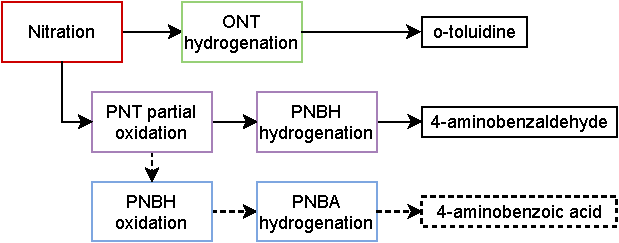
\includegraphics[width=0.8\linewidth]{chapters/0-executive-summary/figures/BFD_nitroma-Page-3.pdf}
    \caption{Simplified synthesis route for Nitroma's process}
    \label{fig:BFD-ES}
\end{wrapfigure}

Firstly, the nitration of toluene with 70\% aqueous nitric acid is carried out in a shell-and-tube heat exchanger reactor packed with H-mordenite catalyst. Solid acid catalysts were preferred over the traditional mixed-acid synthesis due to environmental, safety and performance advantages. Zeolites indeed alleviate the need for costly and energy intensive regeneration of corrosive sulphuric acid, as well as preventing the emission of toxic and global warming potential nitrogen oxides. Heterogeneous catalysis is also attractive from an economical point of view since it favours the more economically desirable \para-nitrotoluene (PNT) isomer. The nitration reactor effluent is fed to a decanter to separate the aqueous nitric acid from the organic phase. Following water evaporation in a distillation column, nitric acid is recycled back into the nitration reactor at a \SI{94}{mol\percent} purity. Meanwhile, the organic phase is sent to a distillation column to recycle unreacted toluene to the nitration reactor. The nitrotoluenes are sent to a second distillation column to separate the more volatile o-nitrotoluene (ONT) from m-nitrotoluene (MNT) and PNT. The large difference in the PNT and MNT melting points is exploited in a mixed-suspension mixed-product removal crystalliser, followed by a hydraulic wash column.

ONT is mixed with methanol and hydrogenated under pressure over Pd/C catalyst to o-toluidine (o-TOL) in a co-current trickle bed reactor operating with both gas and liquid in downflow mode. Trickle bed reactor is chosen due to the ease of operation at high pressure and the relative slow catalyst deactivation, which is imperative for an expensive catalyst usage. o-TOL is then purified to achieved a purity of \SI{99.4}{mol\percent}. The hydrogen gas leaves the reactor via an outlet port, and the effluent enters a distillation column to separate methanol and water from the less volatile organic compounds. Methanol is further distilled to be recycled to teh reactor.

Meanwhile, PNT is fed into an oxidation reactor packed with cobalt , currently operated in parallel, to produce either 4-NBH or 4-NBA. In an effort of plant modularity, Nitroma aims to redesign the oxidation reactors to be operated in series to reduce the CAPEX and the loss of unreacted reactants. The PNT melts in the reactor and is mixed with air. Oxidation of PNT takes place in packed-bed microreactor with cobalt phthalocyanine catalyst, operating at \SI{750}{\K} and \SI{0.5}{\atm} for 4-NBH production (R301), and \SI{483}{\K} and \SI{0.5}{\atm} for 4-NBA production (R302). The reason for the difference in operating conditions have been detailed earlier in Section \ref{4-NTox}.

Nitroma's modular reactor design results in two different reactor effluents depending on whether 4-NBH is the major product (ABH scenario) or 4-NBA (ABA scenario). In both scenarios, the effluent from R301/R302 is sent to a flash drum (S301) that removes air and water vapour from the organic stream, which is then fed into a distillation column (S302), where \SI{99.9}{mol\percent} of the unreacted PNT is separated from the less volatile nitroaromatics. 

In the 4-ABA scenario, the separated PNT stream also contains 4-NBH and water. These chemicals are separated in a second distillation column (S303), yielding a \SI{93}{mol\percent} pure PNT stream which can be sold as a by-product and a \SI{58.9}{mol\percent} pure 4-NBH stream. Future work will recycle the 4-NBH to the second oxidation reactor (R302) to be converted to 4-NBA.

The effluent from the 4-NBH reactor (R301) contains \SI{9.7}{mol\percent} of 4-NBA, of which \SI{99.9}{mol\percent} is separated from the more volatile compounds in S302. The lighter PNT, 4-NBA and water are separated in column S303, yielding a \SI{99.9}{mol\percent} pure 4-NBA stream and a waste stream containing PNT and water. Future work will recycle the unreacted PNT into the oxidation reactors.



 

